\begin{frame}{Информация о предприятии}
    \begin{columns}
        \column{0.5\textwidth}
            \begin{itemize}
                \item 15 лет на рынке
                \item Офисы в России, Великобритании, Чехии и других странах
                \item Портал SecurityLab.ru
                \item Научно-практический форум Positive Hack Days
            \end{itemize}
        \column{0.5\textwidth}
            \begin{figure}[h!]
                \centering
                
\includegraphics[width=1\textwidth]{pt_logo}
                \label{img:pt_logo}
            \end{figure}
    \end{columns}
\end{frame}

\begin{frame}{Информация о предприятии. Продукты}
    \begin{columns}
        \column{0.5\textwidth}
            \begin{itemize}
                \item MaxPatrol 8
                \item MaxPatrol SIEM
                \item PT Application Firewall
                \item PT Application Inspector
                \item PT MultiScanner
                \item XSpider
                \item PT ISIM
            \end{itemize}
        \column{0.5\textwidth}
            \begin{figure}[h!]
                \centering
                
\includegraphics[width=1\textwidth]{pt_logo}
                \label{img:pt_logo}
            \end{figure}
    \end{columns}
\end{frame}

\begin{frame}{Безопасность АСУ ТП}
    Количество компонентов АСУ ТП, доступных в сети Интернет
    \begin{figure}[h!]
        \centering
        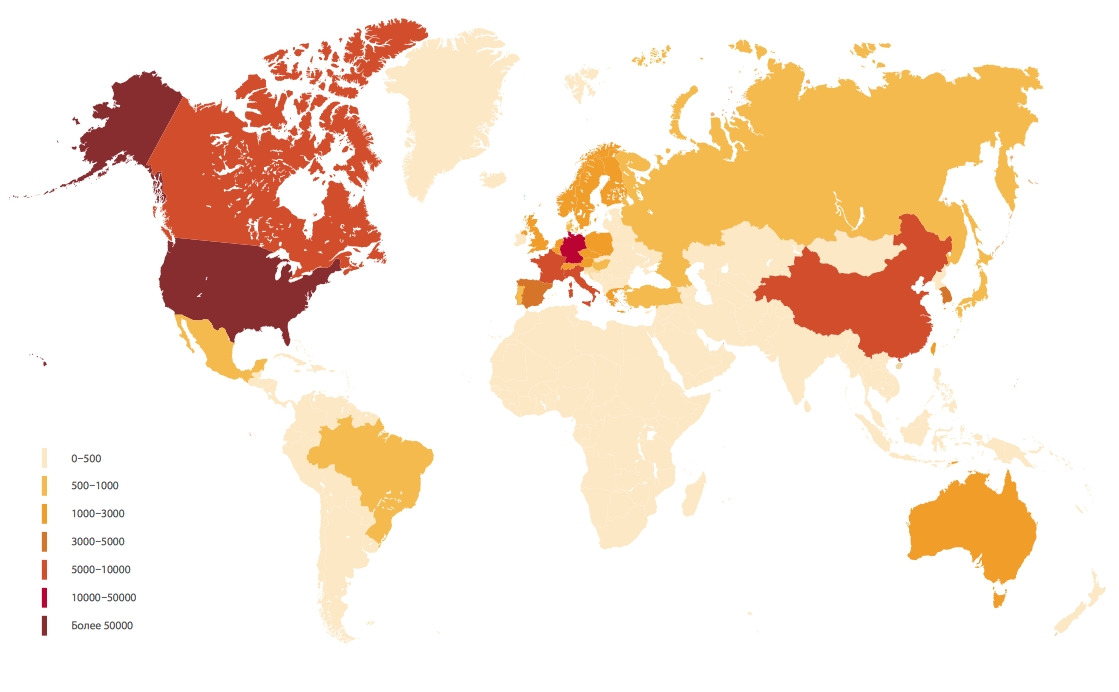
\includegraphics[width=1\textwidth]{world_map}
        \label{img:world_map}
    \end{figure}
\end{frame}

\begin{frame}{PT ISIM. Industrial Security Incident Manager}
    \begin{columns}
        \column{0.5\textwidth}
            \begin{itemize}
                \item Система управления инцидентами кибербезопасности
                \item Анализ копии трафика промышленной сети
                \item Выявление внутренних и внешних угроз
            \end{itemize}
        \column{0.5\textwidth}
            \begin{figure}[h!]
                \centering
                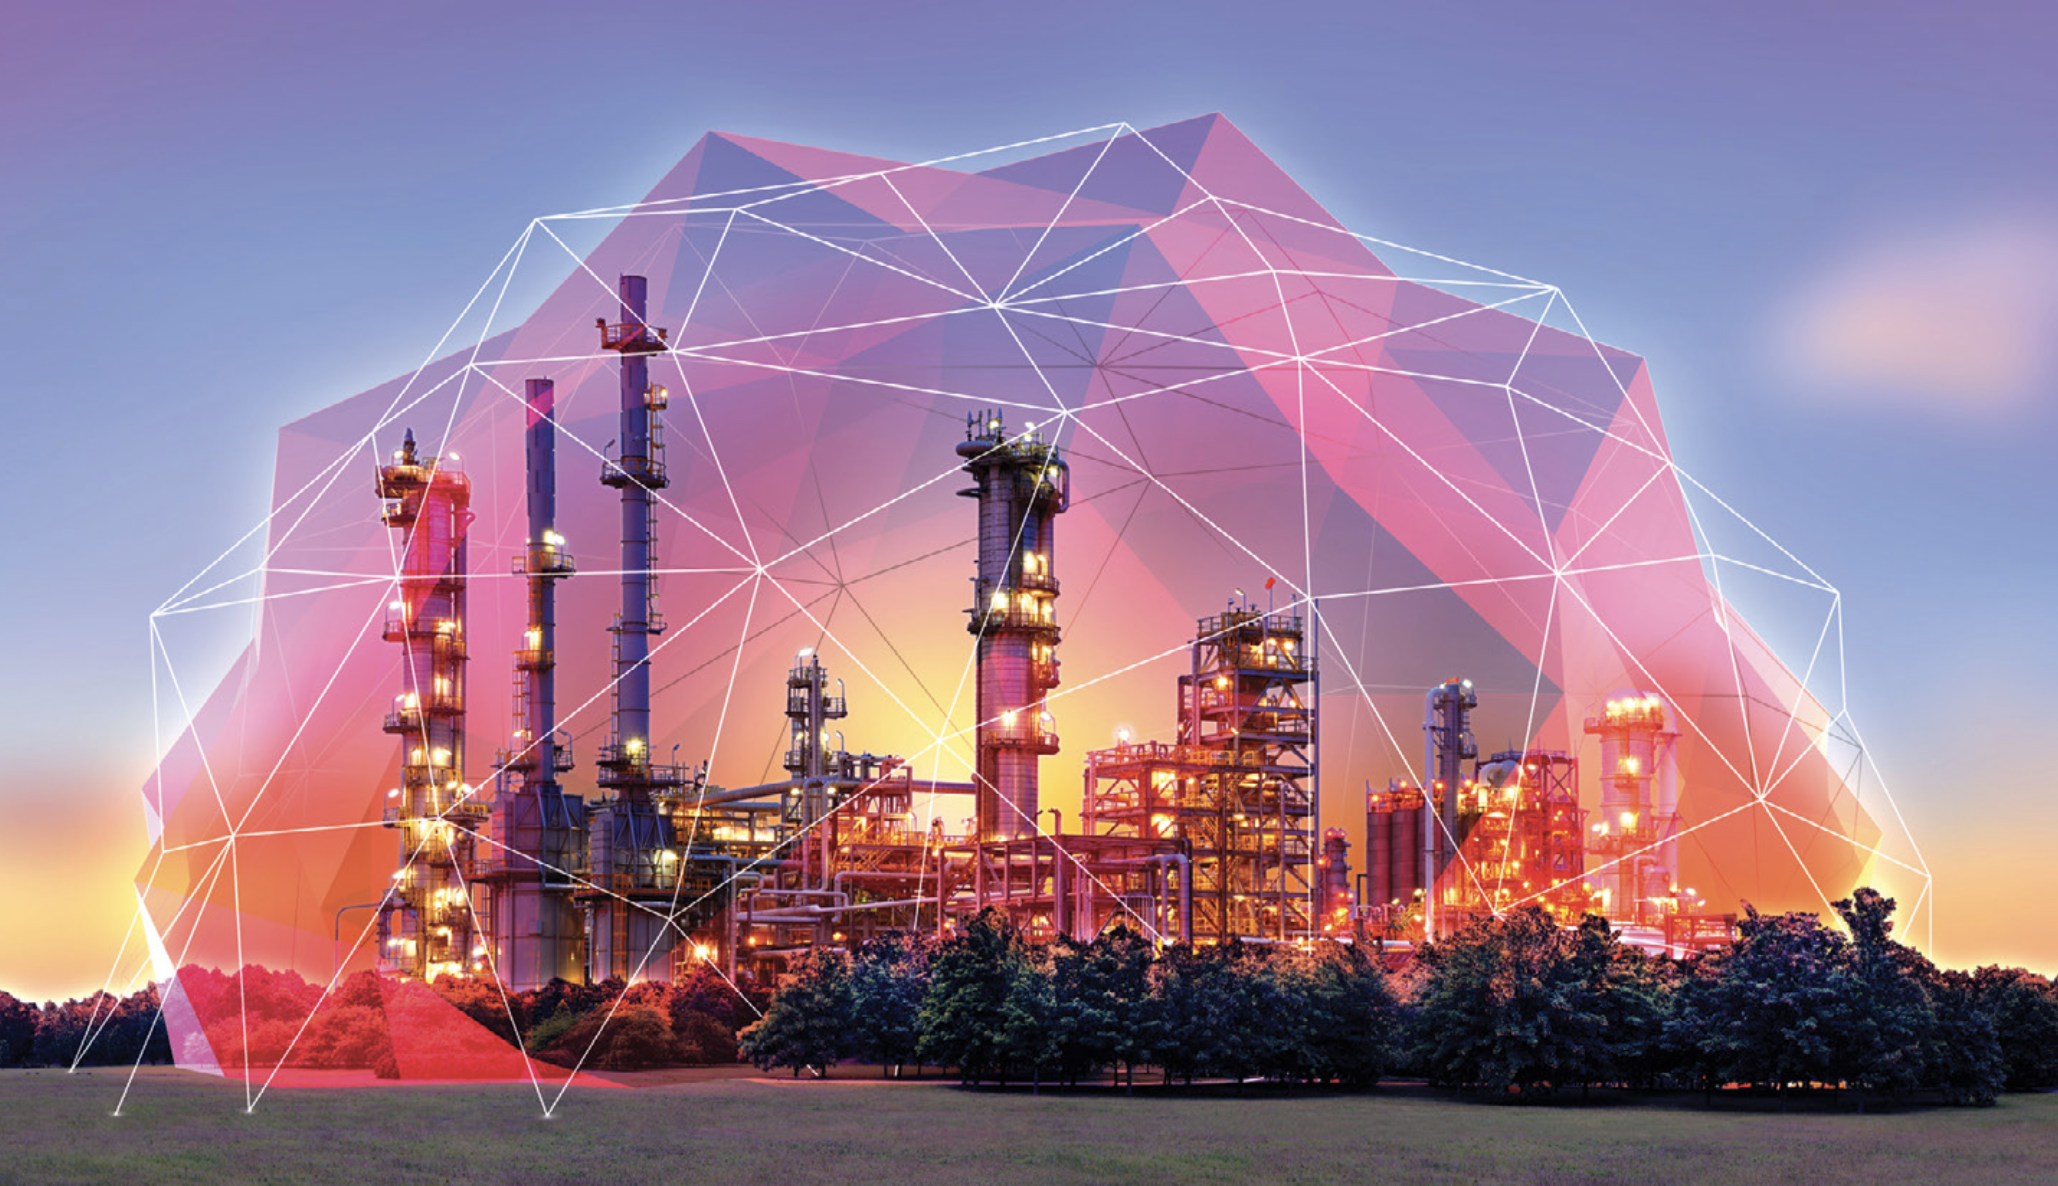
\includegraphics[width=1\textwidth]{pt_isim_logo}
                \label{img:pt_isim_logo}
            \end{figure}
    \end{columns}
\end{frame}

\begin{frame}{PT ISIM. Компоненты}

    \begin{figure}[h!]
        \centering
        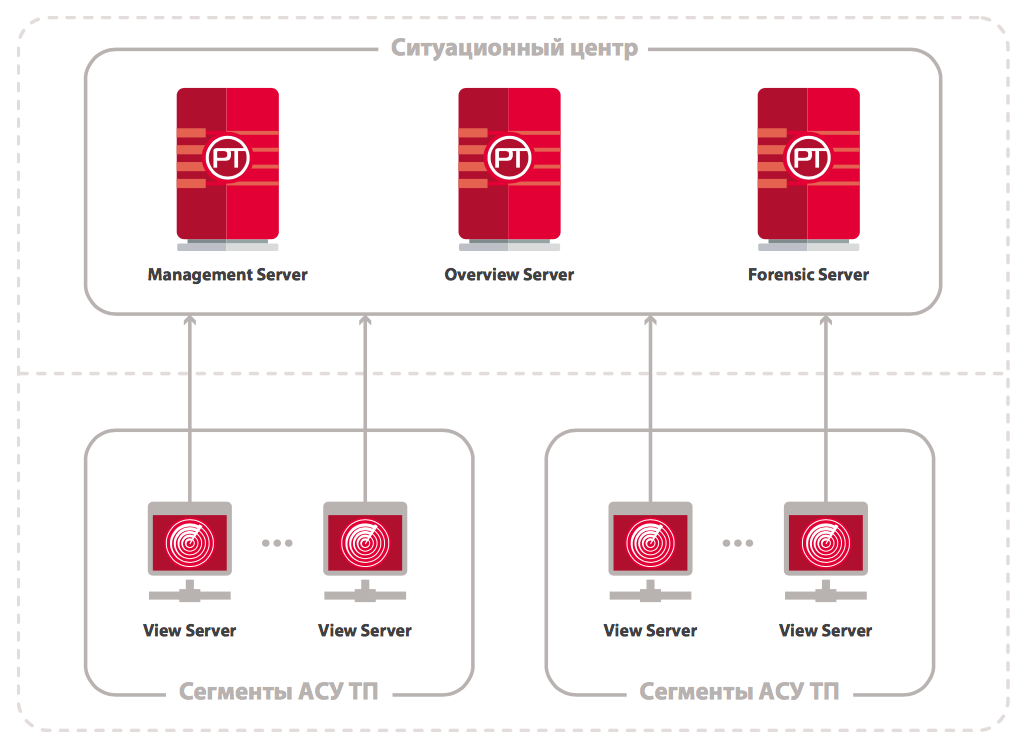
\includegraphics[width=1\textwidth]{components}
        \label{img:components}
    \end{figure}
\end{frame}

\begin{frame}{PT ISIM. Примеры внедрения}
    \begin{figure}[h!]
        \centering
        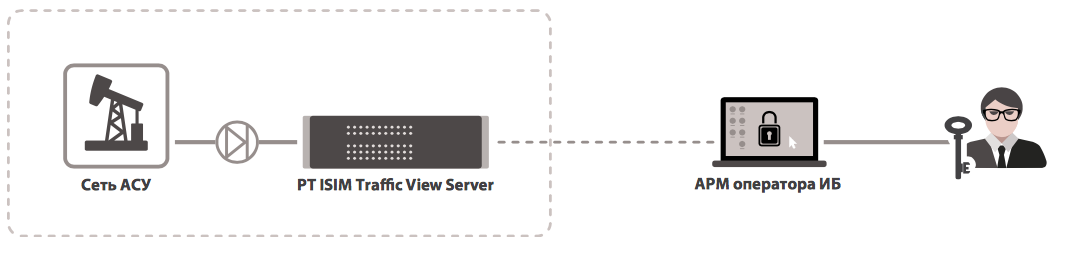
\includegraphics[width=1\textwidth]{int_example_1}
        \label{img:int_example_1}
    \end{figure}
    \begin{figure}[h!]
        \centering
        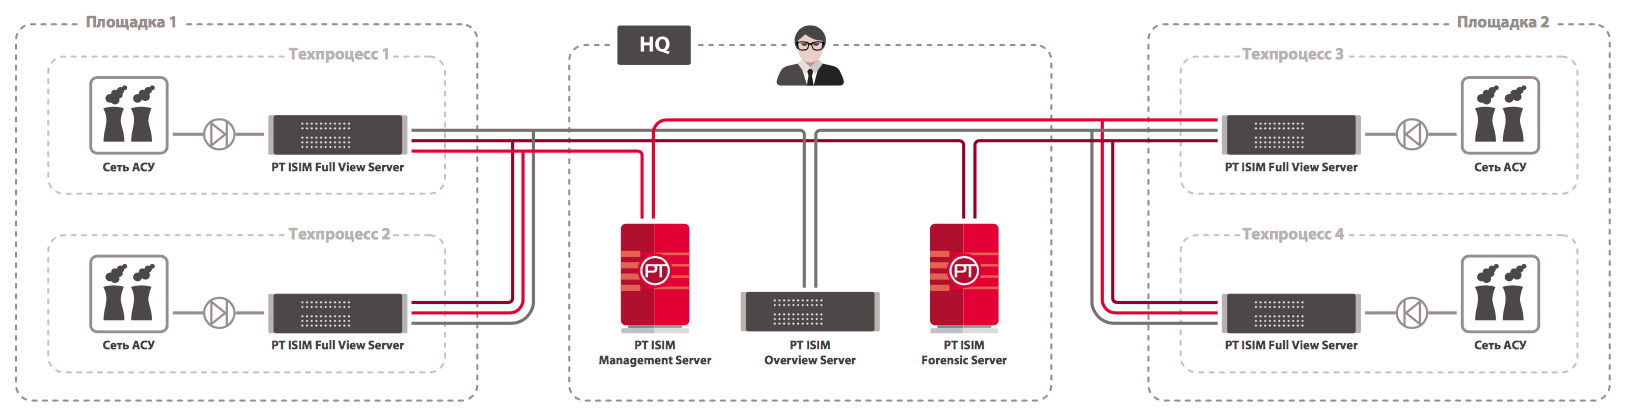
\includegraphics[width=1\textwidth]{int_example_2}
        \label{img:int_example_2}
    \end{figure}
\end{frame}

\begin{frame}{Подходы к тестированию}
    \begin{itemize}
        \item Функциональное тестирование
        \item Нагрузочное тестирование
        \item Стресс-тестирование
        \item Компонентное тестирование
        \item Интеграционное тестирование
        \item Smoke-тестирование
        \item Регрессионное тестирование
    \end{itemize}
\end{frame}

\begin{frame}{Py.test}
    \begin{columns}
        \column{0.5\textwidth}
            \begin{itemize}
                \item Набор библиотек для автоматизации тестирования
                \item Подробный отчёт
                \item Параметризация тестов
                \item Метки для маркировки тестов
                \item Большое количество дополнительных модулей
            \end{itemize}
        \column{0.5\textwidth}
            \begin{figure}[h!]
                \centering
                
\includegraphics[width=1\textwidth]{pytest_logo}
                \label{img:pytest_logo}
            \end{figure}
    \end{columns}
\end{frame}

\begin{frame}{Httpapi}
    \begin{columns}
        \column{0.5\textwidth}
            \begin{itemize}
                \item Предоставляет интерфейс для доступа к компонентам PT ISIM
                \item Используется клиентской частью
                \item Используется другими серверами PT ISIM
                \item Работает при помощи методов HTTP
                \item Оперирует данными в формате JSON
            \end{itemize}
        \column{0.5\textwidth}
            \begin{figure}[h!]
                \centering
                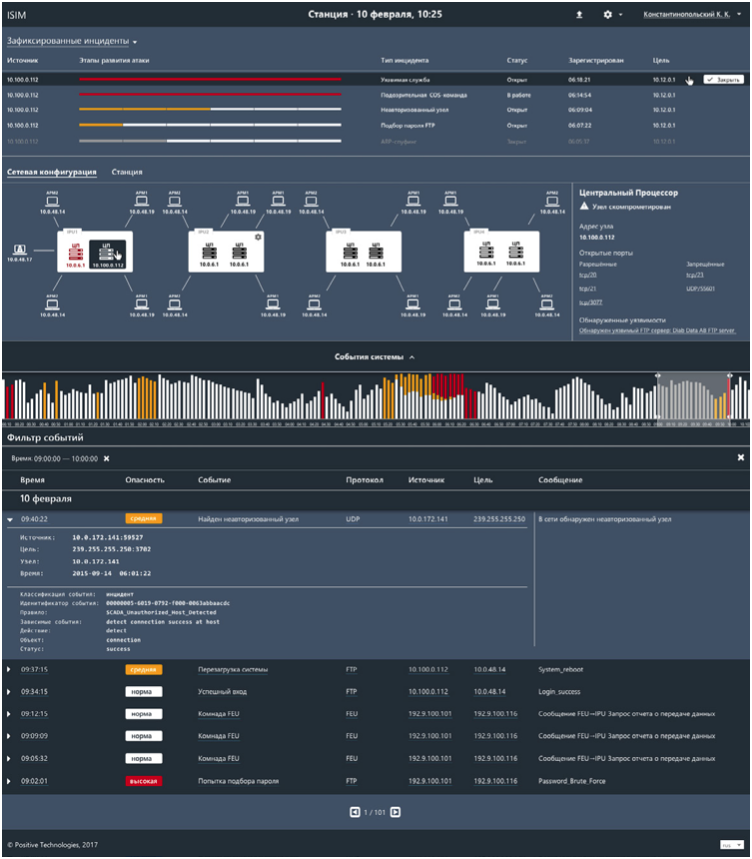
\includegraphics[width=1\textwidth]{08}
                \label{img:web_ui}
            \end{figure}
    \end{columns}
\end{frame}

\begin{frame}{Параметризация}
    \begin{columns}
        \column{0.5\textwidth}
            \begin{itemize}
                \item Количество методов httpapi не постоянно
                \item Пользователи и группы изменяются в процессе разработки
                \item Требуется отчёт о каждой проверке каждого метода httpapi для каждого пользователя
            \end{itemize}
        \column{0.5\textwidth}
            \begin{figure}[h!]
                \centering
                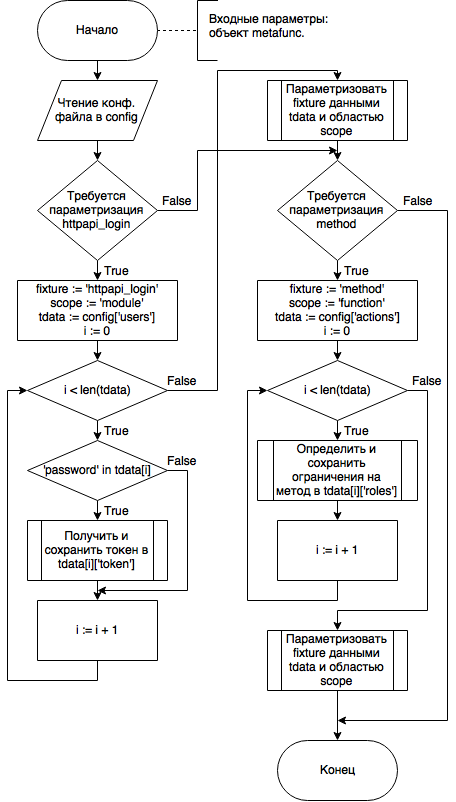
\includegraphics[width=0.8\textwidth]{parametrize_scheme}
                \label{img:parametrize_scheme}
            \end{figure}
    \end{columns}
\end{frame}

\begin{frame}{Конфигурационный файл}
    \begin{columns}
        \column{0.5\textwidth}
            \begin{itemize}
                \item Роли пользователей
                \item Пользователи
                \item Методы httpapi
                \item Ограничения методов
            \end{itemize}
            \begin{figure}[h!]
                \centering
                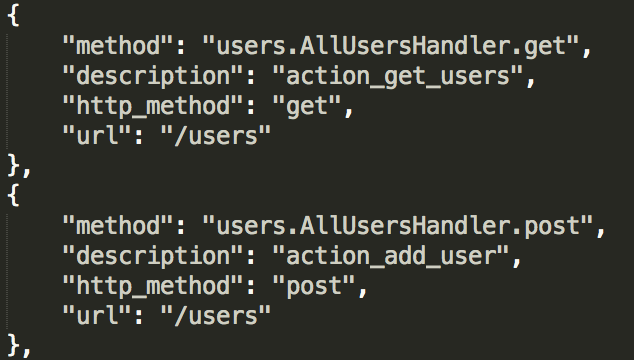
\includegraphics[width=0.8\textwidth]{config_methods}
                \label{img:config_methods}
            \end{figure}
        \column{0.5\textwidth}
            \begin{figure}[h!]
                \centering
                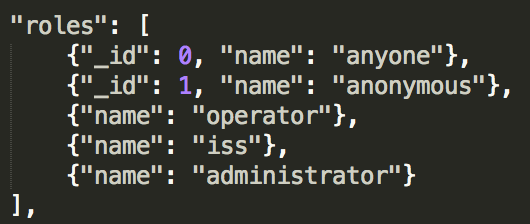
\includegraphics[width=0.8\textwidth]{config_roles}
                \label{img:config_roles}
            \end{figure}
            \begin{figure}[h!]
                \centering
                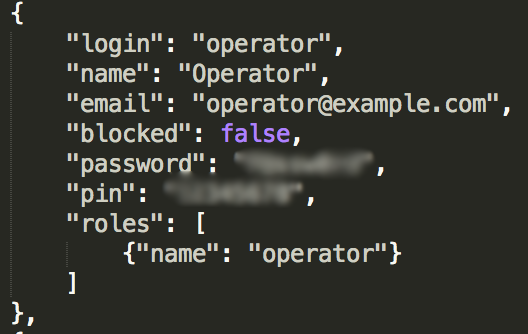
\includegraphics[width=0.8\textwidth]{config_user_operator}
                \label{img:config_user_operator}
            \end{figure}
    \end{columns}
\end{frame}

\begin{frame}{Описание программы}
    \begin{columns}
        \column{0.5\textwidth}
            \begin{itemize}
                \item Сопоставление методов httpapi с ограничениями прав
                \item Параметризация входных данных
                \item Тестирование методов httpapi
            \end{itemize}
        \column{0.5\textwidth}
            \begin{figure}[h!]
                \centering
                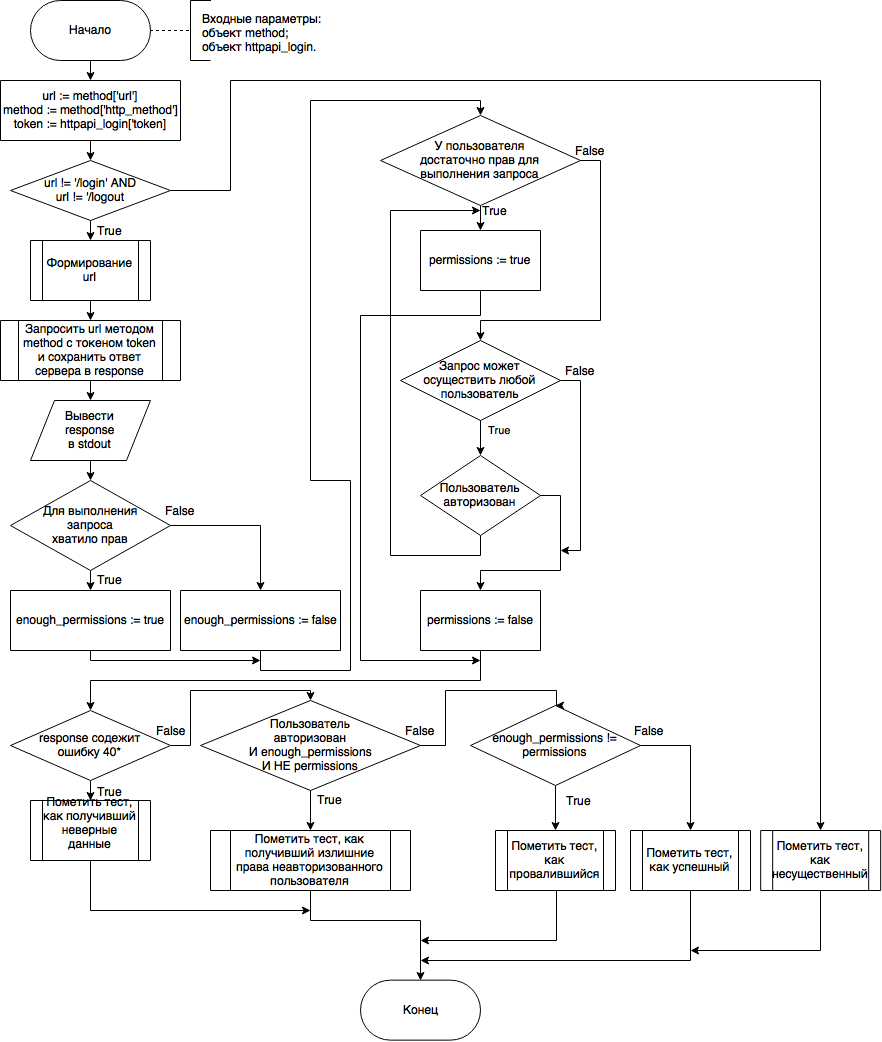
\includegraphics[width=0.9\textwidth]{test_method_scheme}
                \label{img:test_method_scheme}
            \end{figure}
    \end{columns}
\end{frame}

\begin{frame}{Работа программы}
    \begin{columns}
        \column{0.5\textwidth}
            \begin{itemize}
                \item Информация о работе программы в stdout
                \item Определение некорректных ответов httpapi
                \item Определение избыточных прав неавторизованного пользователя
                \item Определение уже сделанных проверок в рамках других тестов
            \end{itemize}
        \column{0.5\textwidth}
            \begin{figure}[h!]
                \centering
                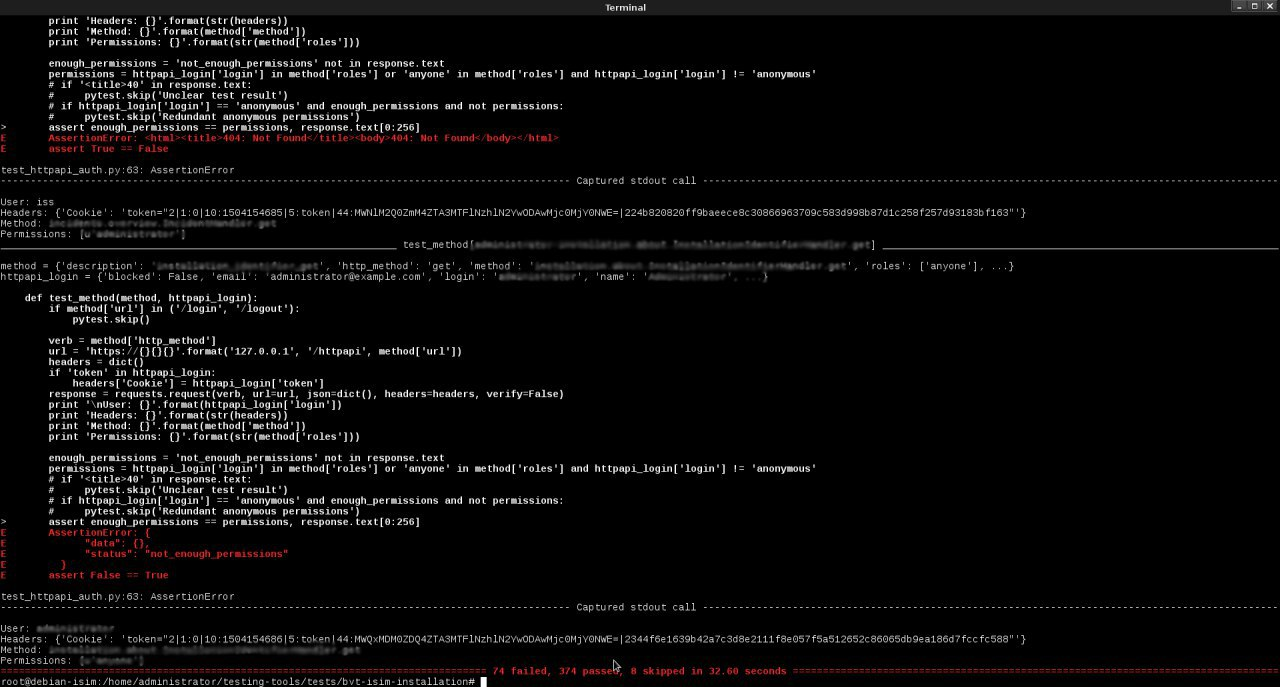
\includegraphics[width=1\textwidth]{test_run}
                \label{img:test_run}
            \end{figure}
    \end{columns}
\end{frame}

\begin{frame}{Результаты работы программы}
    \begin{columns}
        \column{0.5\textwidth}
            \begin{itemize}
                \item Получение html-страниц вместо документов JSON
                \item Наличие недопустимых прав у неавторизованного пользователя
                \item Отсутствие необходимых прав у ряда пользователей
                \item Информирование разработчиков обо всех найденных ошибках при помощи JIRA
            \end{itemize}
        \column{0.5\textwidth}
            \begin{figure}[h!]
                \centering
                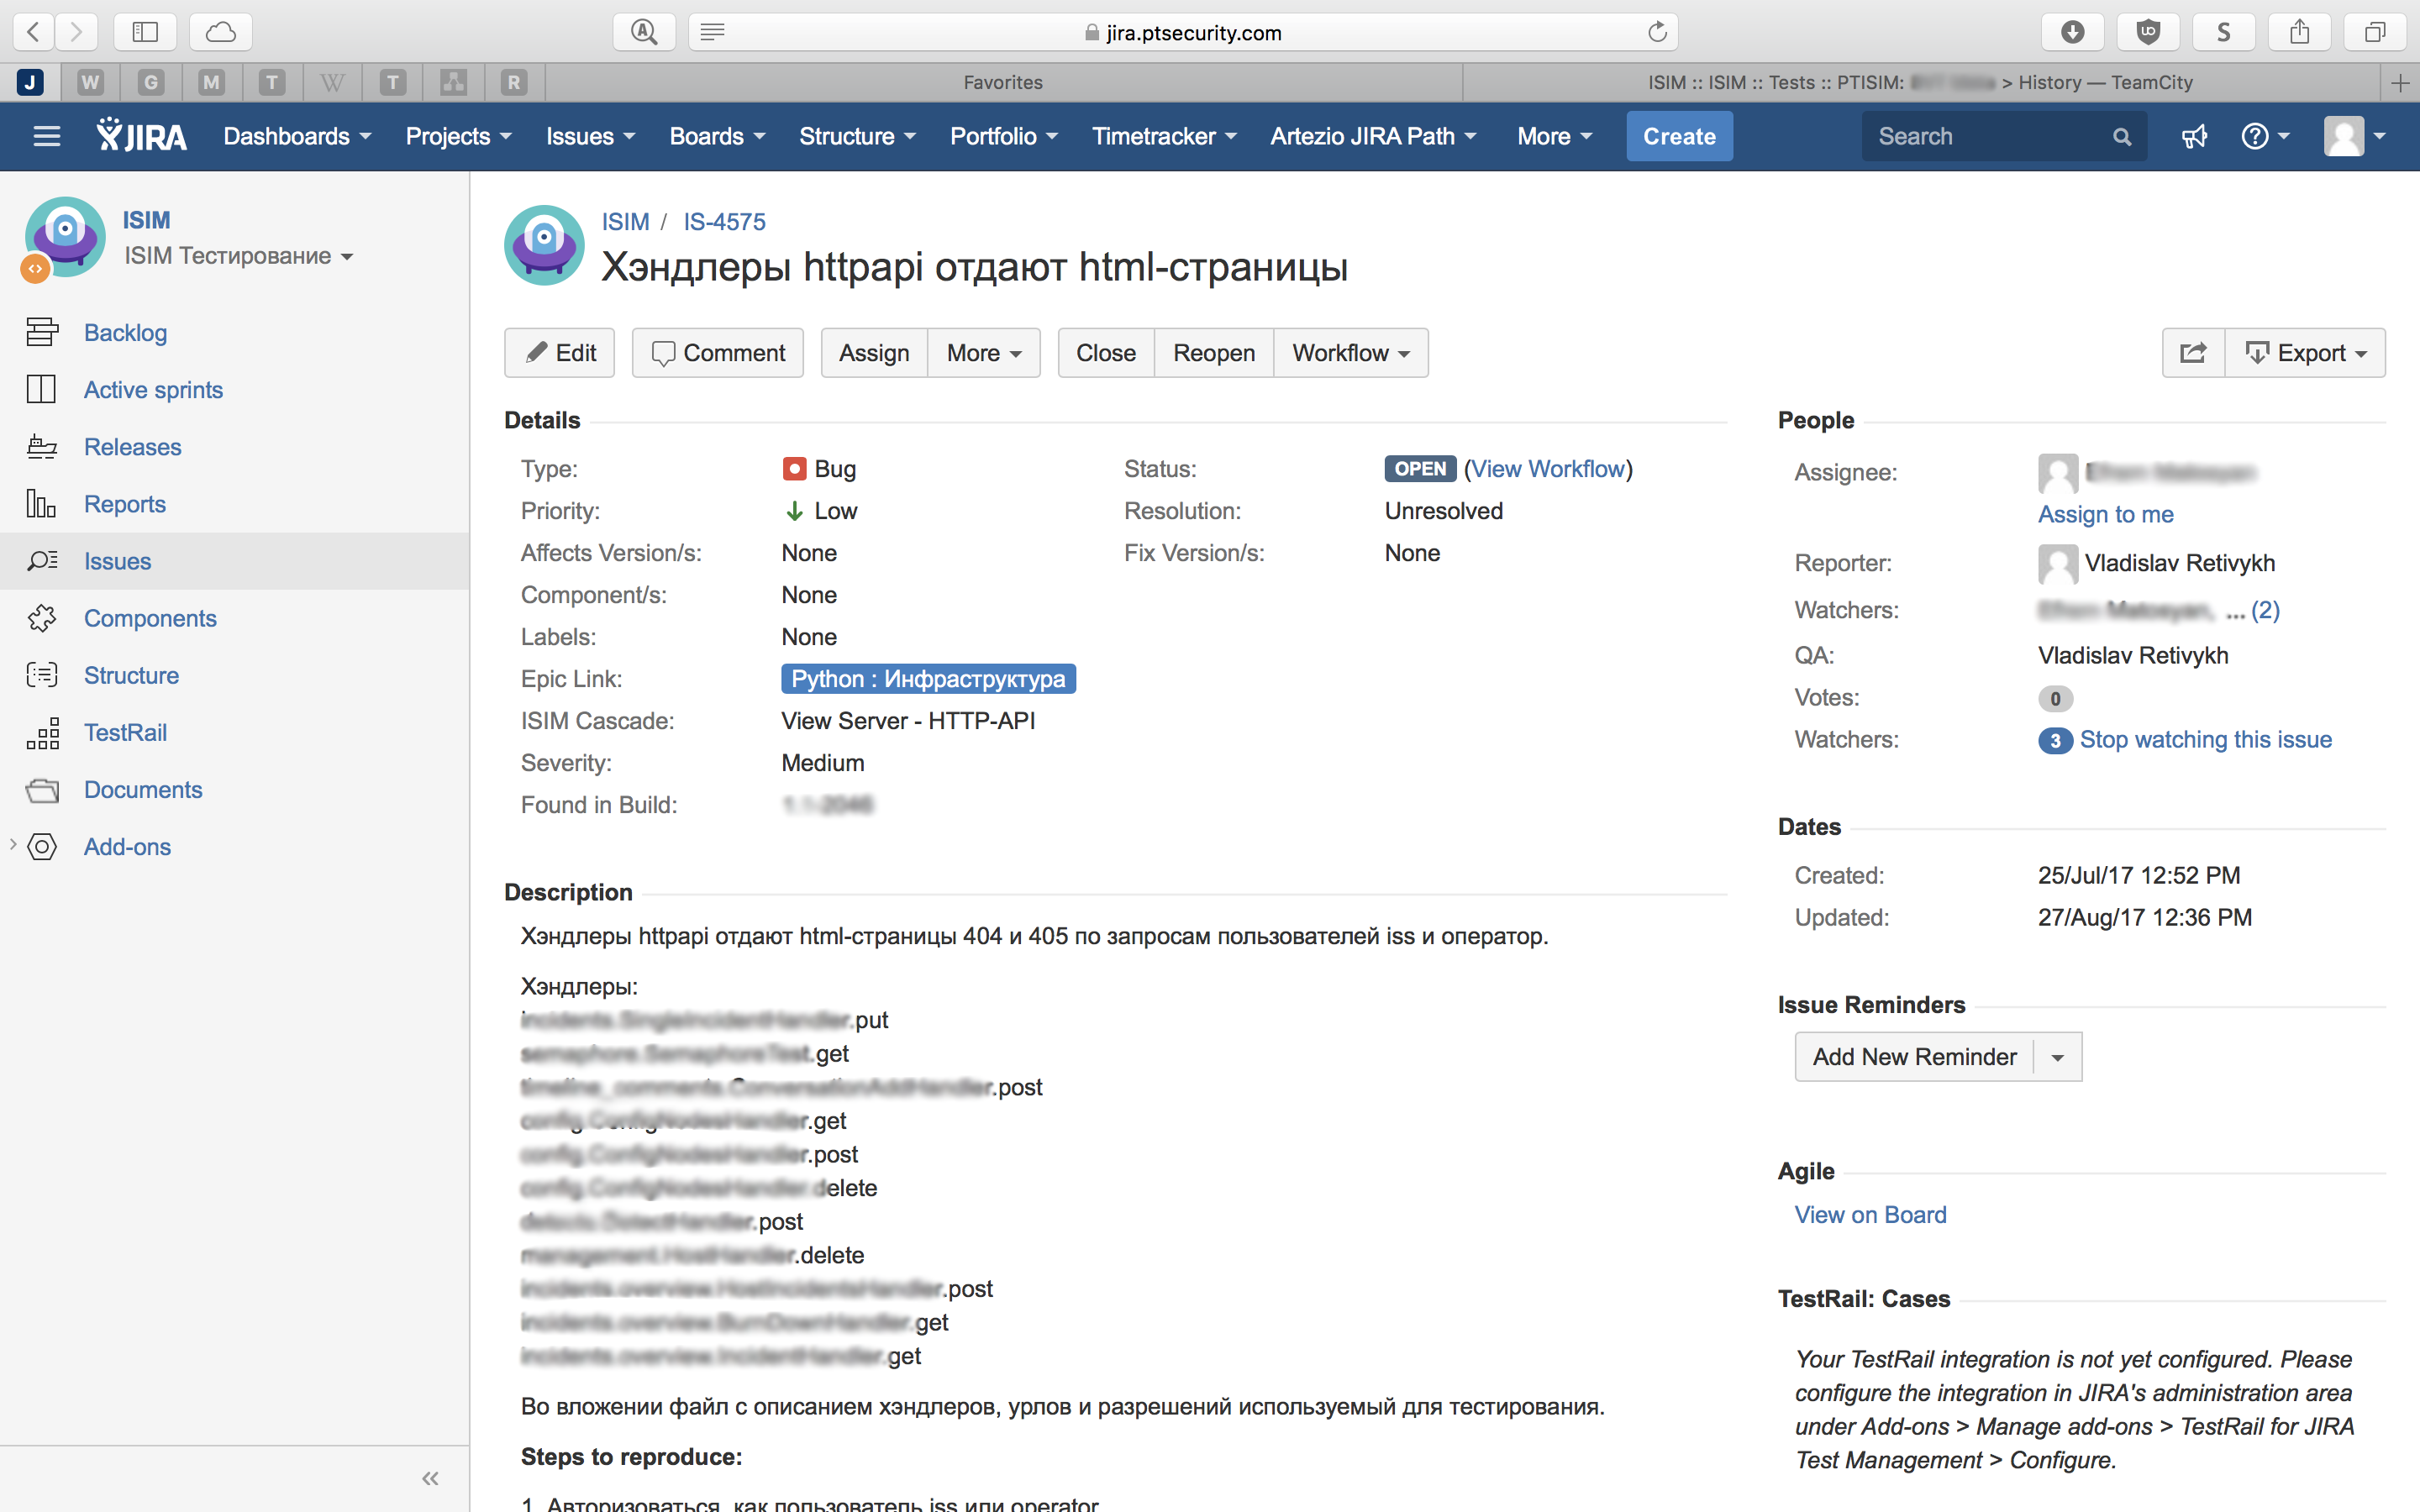
\includegraphics[width=1\textwidth]{jira_40x}
                \label{img:jira_40x}
            \end{figure}
    \end{columns}
\end{frame}

\begin{frame}{Непрерывная интеграция}
    \begin{columns}
        \column{0.5\textwidth}
            \begin{itemize}
                \item Интеграция в уже существующий набор автотестов
                \item Непрерывная интеграция при помощи сервера TeamCity
                \item Автоматическая проверка прав доступа для каждой новой сборки PT ISIM
            \end{itemize}
        \column{0.5\textwidth}
            \begin{figure}[h!]
                \centering
                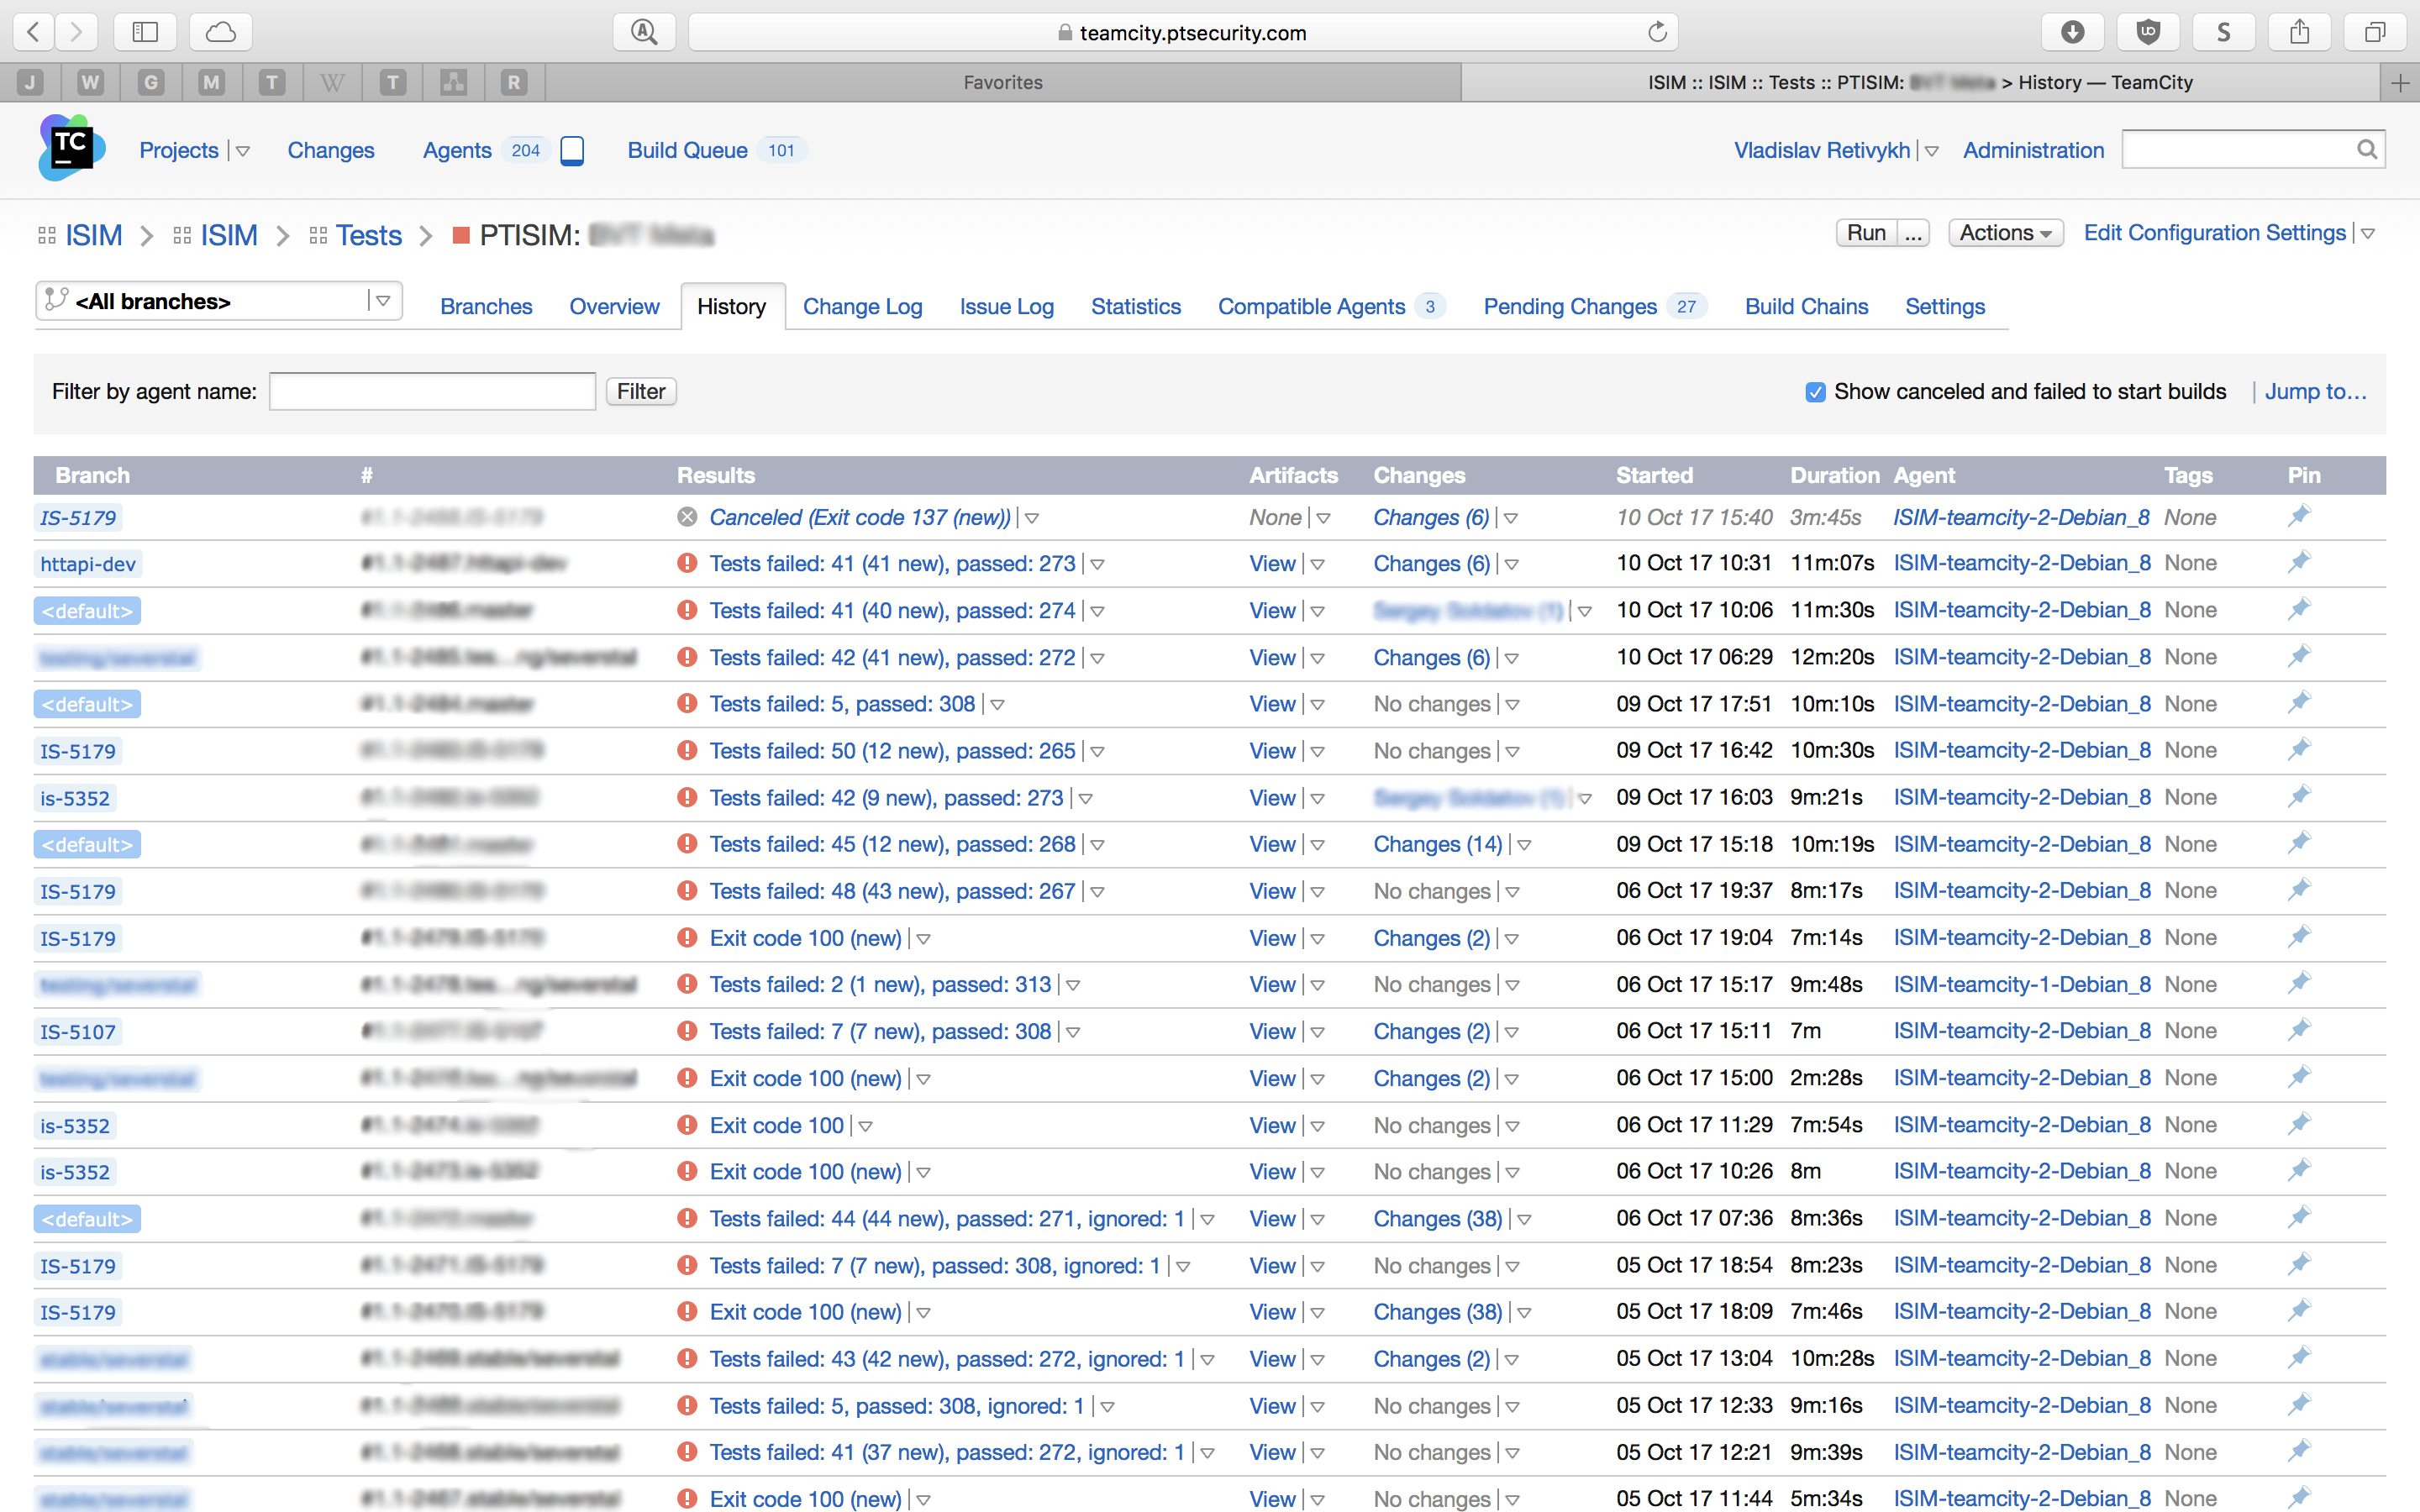
\includegraphics[width=1\textwidth]{teamcity}
                \label{img:teamcity}
            \end{figure}
    \end{columns}
\end{frame}

\begin{frame}{Результаты}
    \begin{itemize}
        \item Проведён анализ конфигурационных файлов PT ISIM
        \item Разработано ПО для проверки политик разграничения доступа к программным интерфейсам
        \item Разработанное ПО интегрировано в существующую систему автотестов
        \item Выявлено 74 несоответствия фактических прав эталонным
    \end{itemize}
\end{frame}

\begin{frame}{Заключение}
    \begin{itemize}
        \item Изучена СУИК PT ISIM
        \item Получены навыки тестирования коммерческого ПО
        \item Получены навыки работы с py.test
        \item Разработанное в рамках практики ПО включено в процесс разработки PT ISIM
    \end{itemize}
\end{frame}